% ==========================================
% Archivo: sections/4_results_and_discussion.tex
% ==========================================
\section{Resultados y Discusión}

\subsection{Comparación y optimización de modelos}

En este apartado se exponen las trayectorias de un cuerpo siendo proyectado con una velocidad $v=700\rm \, m/s$ bajo distintas modelizaciones y ángulos de lanzamiento. Asimismo, también se incluye la optimización del ángulo de lanzamiento para maximizar la distancia recorrida. 

Se comienza mostrando los efectos que tiene, para distintos ángulos, la incorporación de gravedad terrestre variable y rozamiento del aire. En la Figura \ref{fig:ideal_vs_gravedad_vs_aire} se puede observar la trayectoria de un proyectil sometido exclusivamente al efecto de la gravedad constante (izquierda), bajo el efecto de la gravedad variable (centro) y actuando sobre él tanto gravedad variable como el rozamiento del aire (derecha). Para cada uno de los casos, se muestra la trayectoria para un rango de ángulos de 25$^\circ$ a 75$^\circ$.

\begin{figure}[htbp]
    \makebox[\textwidth][c]{%
        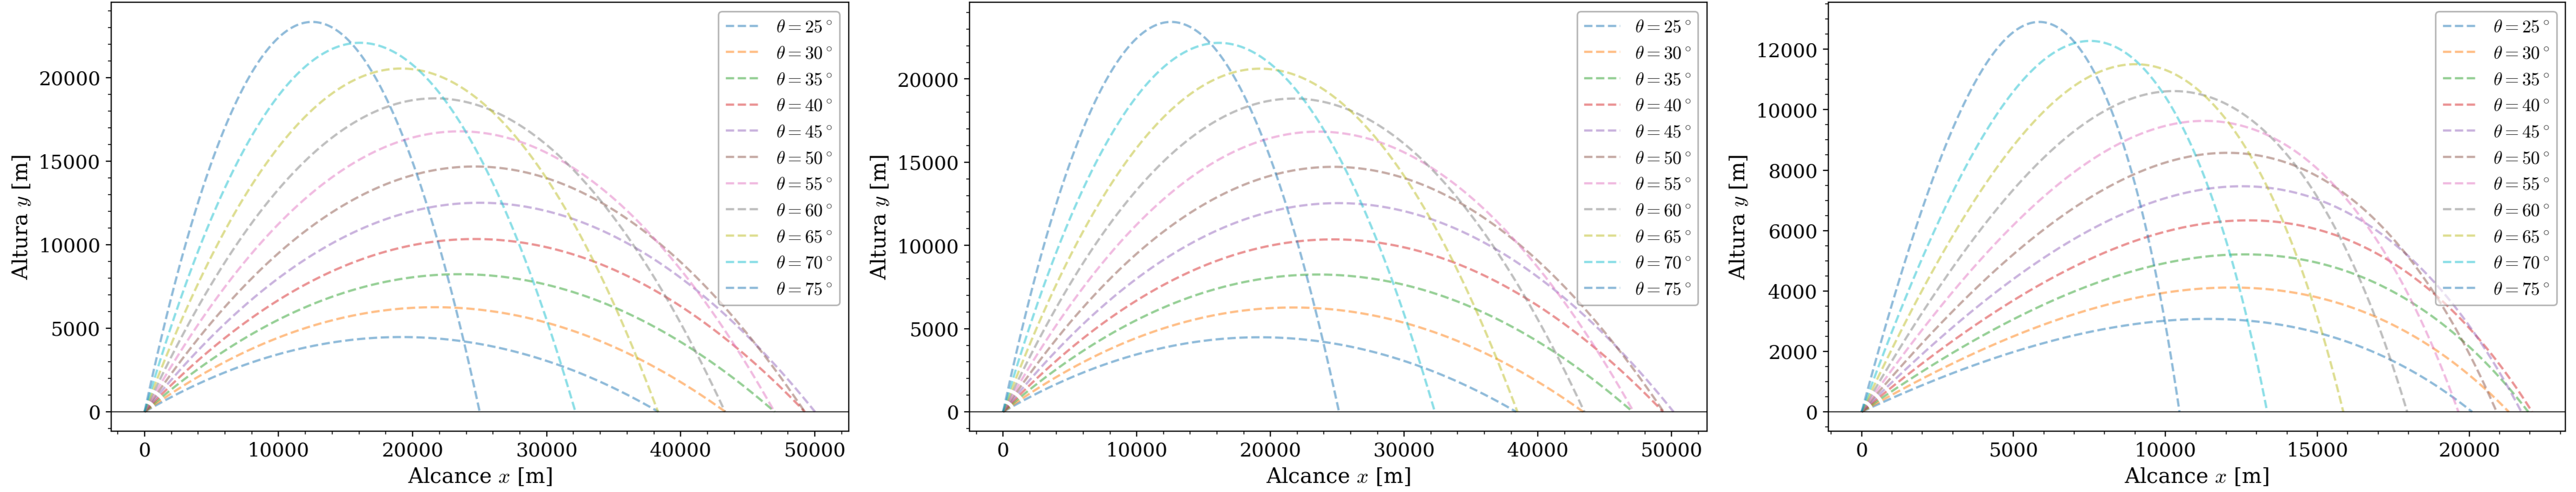
\includegraphics[width=0.95\paperwidth]{figures_tex/ideal_vs_g_vs_air_up.png}%
    }
    \caption{Trayectoria de un proyectil para distintos ángulos y distintos modelos: modelo ideal (izquierda), modelo ideal con gravedad variable en función de la altura (centro), modelo con rozamiento y gravedad variable (derecha).}
    \label{fig:ideal_vs_gravedad_vs_aire}
\end{figure}



Se puede comprobar que el modelo ideal con gravedad variable no presenta una divergencia significativa respecto al modelo ideal, sin embargo, al incluir el rozamiento se produce una fuerte disminución tanto en el alcance como en la altura. En la Figura \ref{fig:comparación}
se muestra cuantitativamente estas diferencias entre la altura máxima y alcance con respecto al caso ideal para los distintos ángulos.

\begin{figure}[htbp]
    \centering
    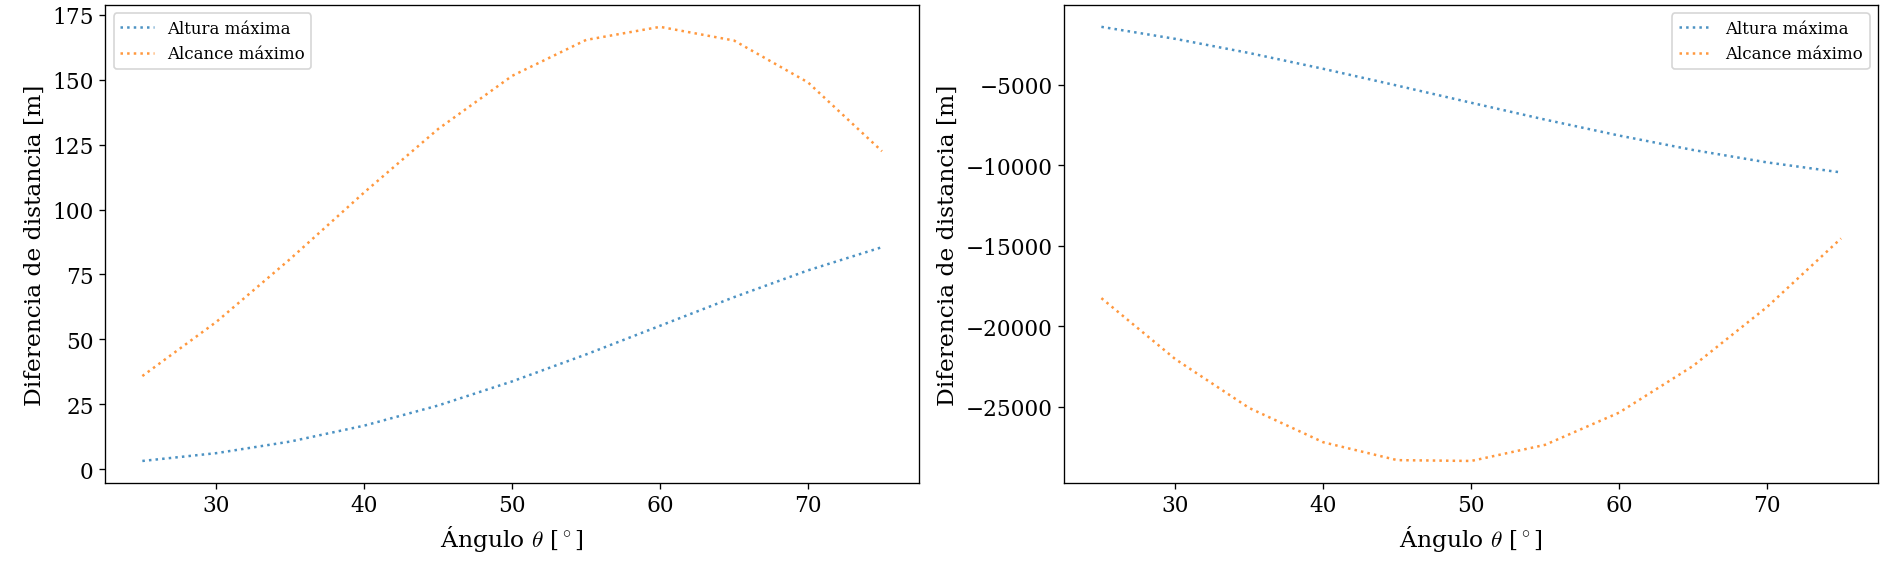
\includegraphics[width=1\linewidth]{figures_tex/ideal_vs_g_vs_air_dn.png}
    \caption{Diferencia de altura máxima y alcance máximo del modelo ideal con gravedad variable (izquierda) o modelo con rozamiento y gravedad variable (derecha) respecto al modelo ideal en función del ángulo de lanzamiento.}
    \label{fig:comparación}
\end{figure}

Resulta evidente que la consideración de gravedad variable ($\Delta \sim 10^{0} - 10^{2} \rm \, m$) tiene un efecto considerablemente menor que el rozamiento con el aire ($\Delta \sim10 ^3- 10^4\, \rm m $). Además, la variación máxima del alcance se observa para un ángulo de $\sim 60^\circ$ en el caso ideal con gravedad variable y para $\sim 48^\circ$ en el modelo con rozamiento. El motivo es que, en el primer supuesto, grandes ángulos permiten alcanzar mayores alturas y por tanto reducir la aceleración en la dirección $y$, dotándole de mayor tiempo al cuerpo para moverse en dirección $x$. Para el segundo supuesto, el rozamiento penaliza largas trayectorias, las cuales se obtienen, en el caso ideal, para ángulos de lanzamiento de $45^\circ$, tal y cómo se muestra en la Tabla \ref{table:optim_all_models}, por lo que las trayectorias previamente óptimas son las que sufren mayor rozamiento. 


En la Figura \ref{fig:all_models_45} se presentan las trayectorias para distintos modelos con un ángulo de lanzamiento de $45^\circ$: caso ideal (sin aire), el único de ellos con gravedad constante; modelo con rozamiento (con aire); modelo isotérmico; modelo adiabático; y efecto Magnus, en el que se considera una rotación en el eje $z$ (perpendicular a la gravedad) y con densidad constante para constreñir las dependencias. Cabe mencionar que en los últimos tres casos, se incluye la contribución del viento $v_{w} = -100 \, \hat{x}\, \rm m/s$. Al igual que se observaba en la Figura \ref{fig:ideal_vs_gravedad_vs_aire}, los modelos isotérmico y adiabático sufren gravemente los efectos del rozamiento con el aire. Resulta curiosa la trayectoria considerando el efecto Magnus, la cual contiene un \textit{loop}. 

\begin{figure}
    \centering
    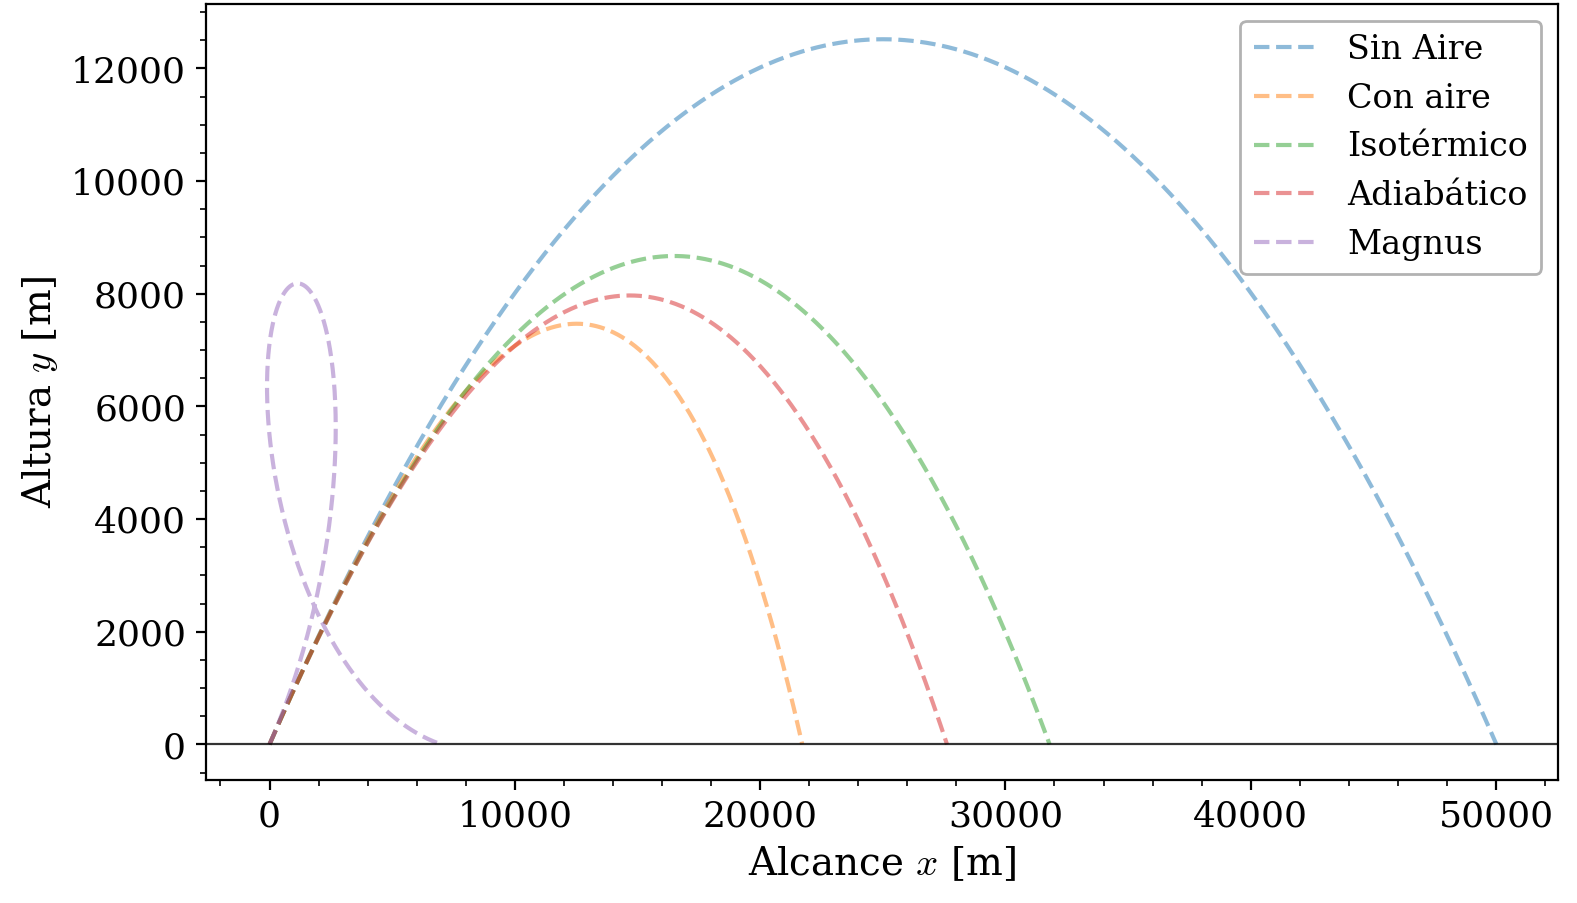
\includegraphics[width=0.82\linewidth]{figures_tex/all_models_45.png}
    \caption{Trayectorias de proyectiles para distintos modelos, con ángulo de lanzamiento $\theta = 45^\circ$.}
    \label{fig:all_models_45}
\end{figure}


Para poder observar mejor la trayectoria del proyectil cuando se considera el efecto Magnus, se muestra en la Figura \ref{fig:magnus_3d} su recorrido en 3D, para un ángulo de lanzamiento $\theta = 30 ^\circ$. Se puede acceder a la animación completa en \href{https://youtu.be/uI-5EuqUfpI}{YouTube}.

\begin{figure}[h!]
    \centering
    \href{https://youtu.be/uI-5EuqUfpI}{
    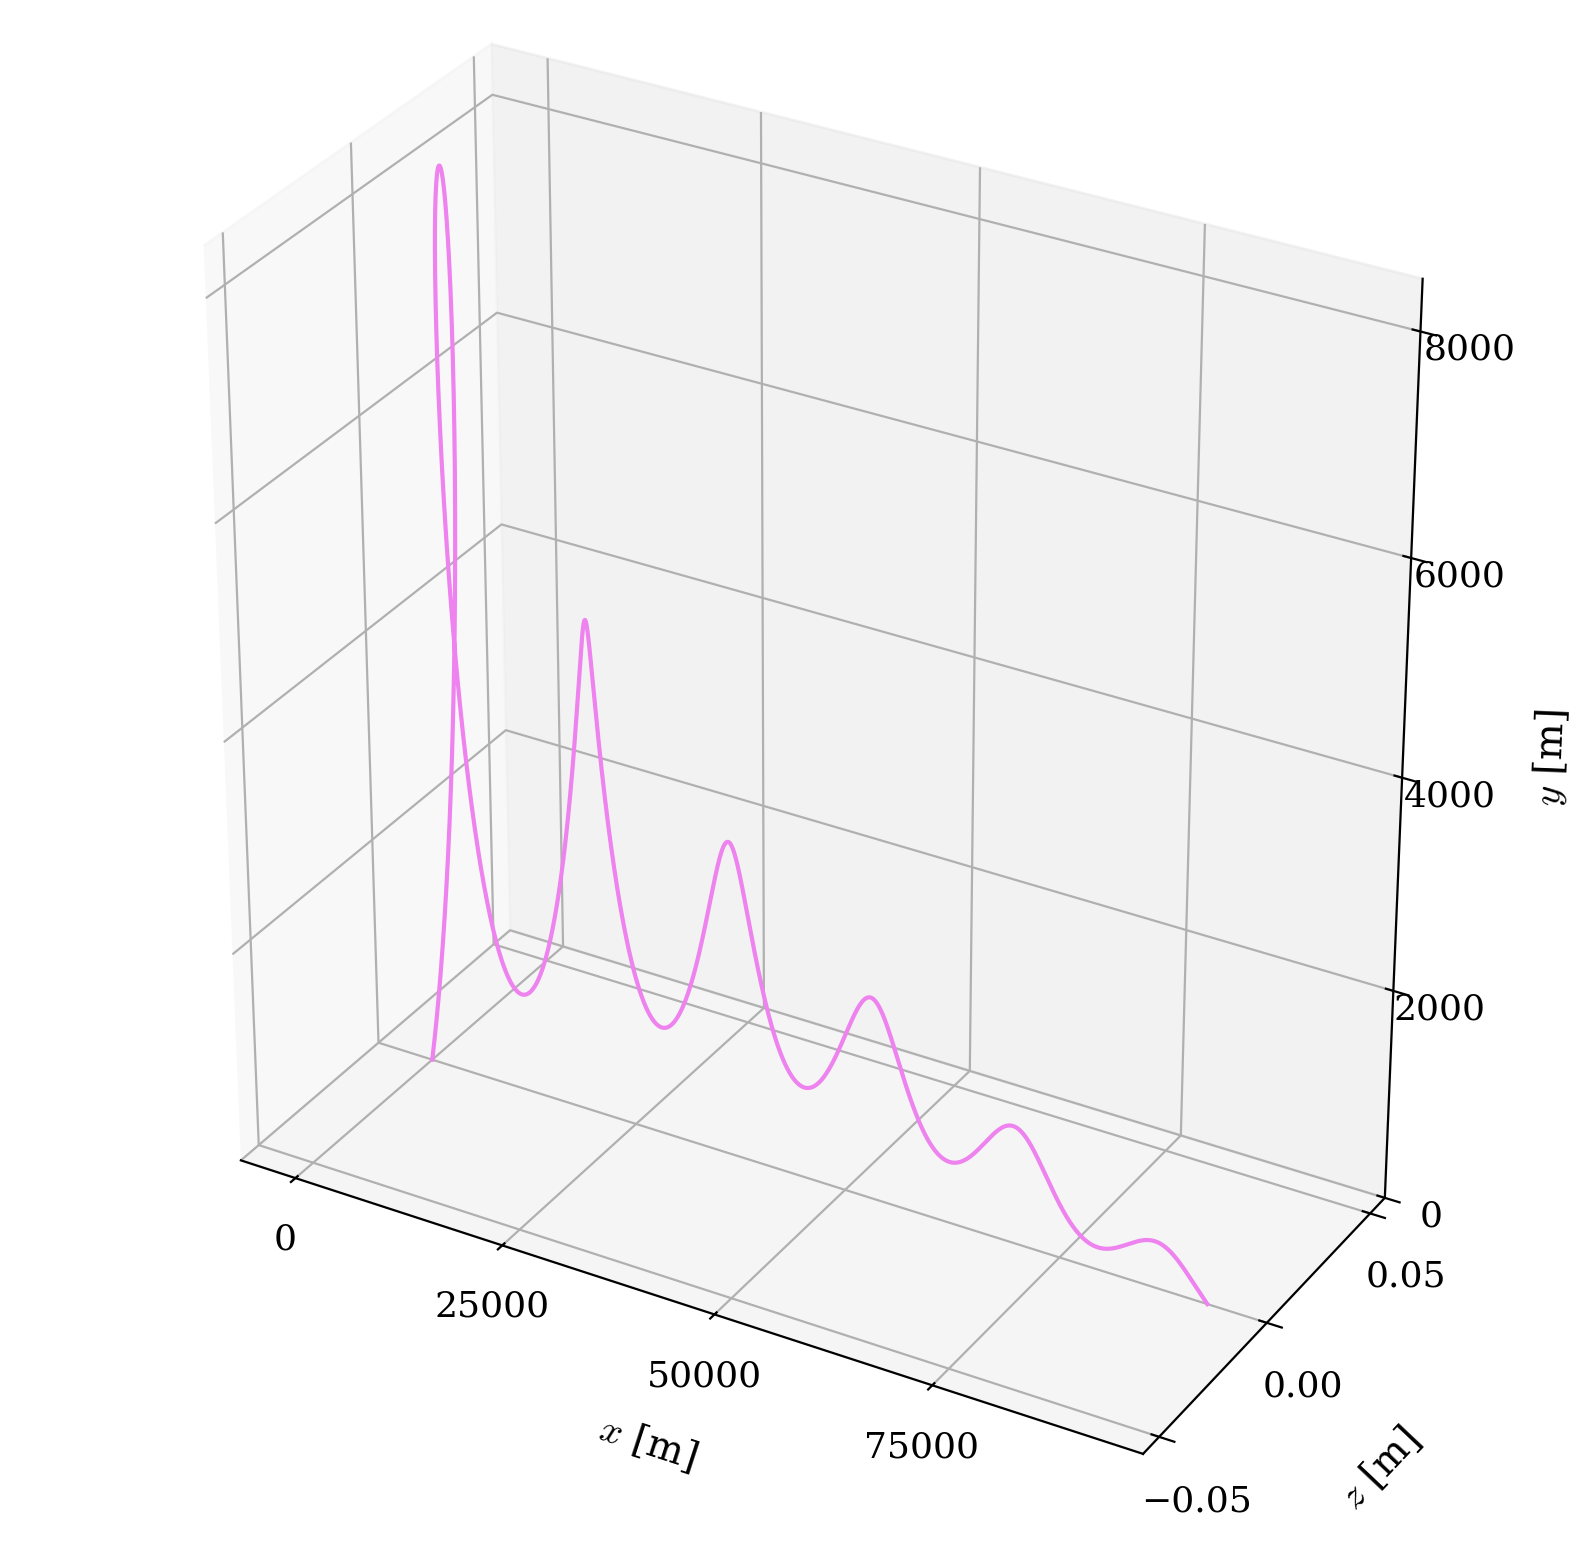
\includegraphics[width=0.7\linewidth]{figures_tex/magnus_3d.png}}
    \caption{Trayectoria de poyectil bajo el efecto Magnus.}
    \label{fig:magnus_3d}
\end{figure}

\newpage


Es de interés estudiar cuáles son los ángulos que maximizan el alcance para los distintos modelos. Estos se presentan en la Tabla \ref{table:optim_all_models}, y se grafican en la Figura \ref{fig:all_models_optim} las trayectorias de los cuerpos bajo los distintos modelos en su ángulo óptimo:
\begin{table}[h]
    \centering
    \caption{Ángulo óptimo para distintos modelos y alcance proyectil.}
    \begin{tabular}{l S[table-format=2.1] S[table-format=6.1]}
        \toprule
        \textbf{Modelo} & {\textbf{Ángulo ($^\circ$)}} & {\textbf{Alcance (m)}} \\ 
        \midrule
        Sin Aire     & 45.0 & 49971.0  \\
        Con Aire    & 38.8 & 22078.2  \\
        Isotérmico & 47.2 & 31876.8  \\
        Adiabático   & 43.7 & 27633.6  \\
        Magnus      & 6.4  & 113092.3 \\
        \bottomrule
    \end{tabular}
    \label{table:optim_all_models}
\end{table}



\begin{figure}[h!]
    \centering
    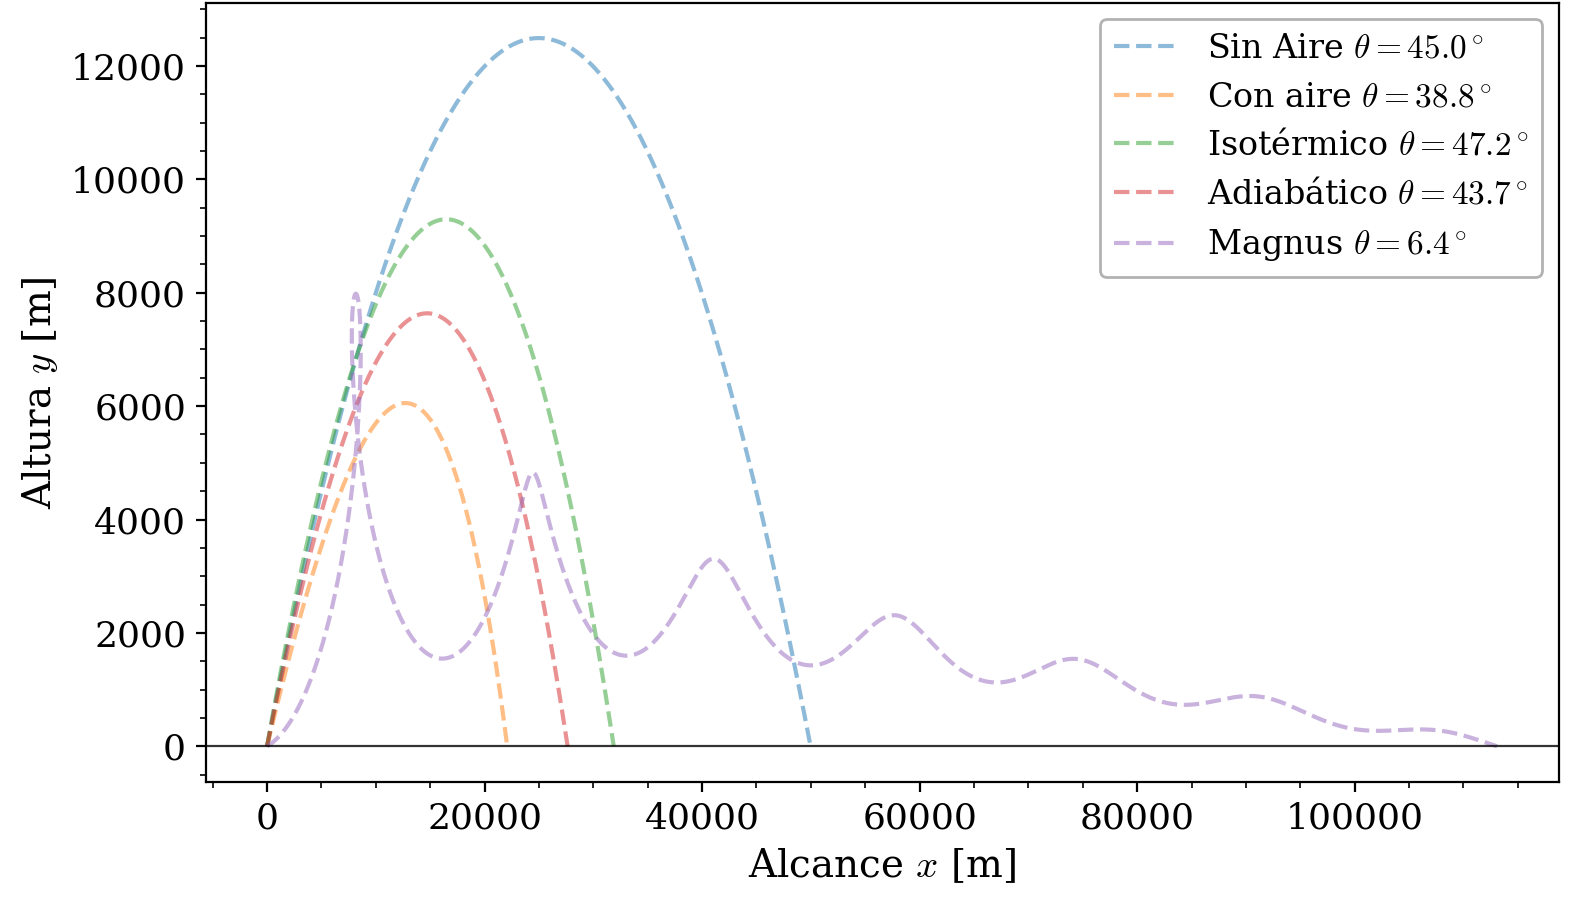
\includegraphics[width=0.82\linewidth]{figures_tex/all_models_optim.png}
    \caption{Trayectorias de proyectiles para distintos modelos con su mejor ángulo de lanzamiento.}
    \label{fig:all_models_optim}
\end{figure}


Finalmente, se estudia el lanzamiento de una pelota de golf, y en particular, los efectos \textit{slice} y \textit{hook}. Para ello, se considera un régimen adiabático con coeficiente aerodinámico variable según \eqref{eq:coef_arrastre}, gravedad variable en función de la altura, velocidad de viento $v_w = -10\, \hat{x}\rm\, m/s$ y rotación $\boldsymbol{\omega} = \omega \, \hat{k}$. Para conseguir el efecto \textit{slice} se requiere $\omega >0$, mientras que para conseguir el efecto \textit{hook} es necesario $\omega <0$. Realizando un análisis idéntico al anterior, se determina el ángulo óptimo $\theta_\text{opt} = 34.0^\circ$, el cual provoca una desviación en el eje $y$ de valor $\Delta y= \pm 46.7\, \rm m$. En la Figura \ref{fig:hook_slice} se puede observar la trayectoria de la pelota de golf en estas condiciones. La animación completa está disponible en \href{https://youtu.be/HMuMxsNRagU}{YouTube}.

Nótese que dado que el viento se considera exclusivamente en la dirección del eje $x$, las situaciones para \textit{slice} y \textit{hook} son simétricas respecto al plano $y=0$. También es remarcable el hecho de que, dado que la dirección de rotación de la pelota es distinta (ahora es paralela a la gravedad, antes era perpendicular a la gravedad), no obtenemos \textit{loops} ni giros tales como observábamos en la Figura \ref{fig:magnus_3d}.\vfill


\begin{figure}[h]
    \centering
    \href{https://youtu.be/HMuMxsNRagU}{
    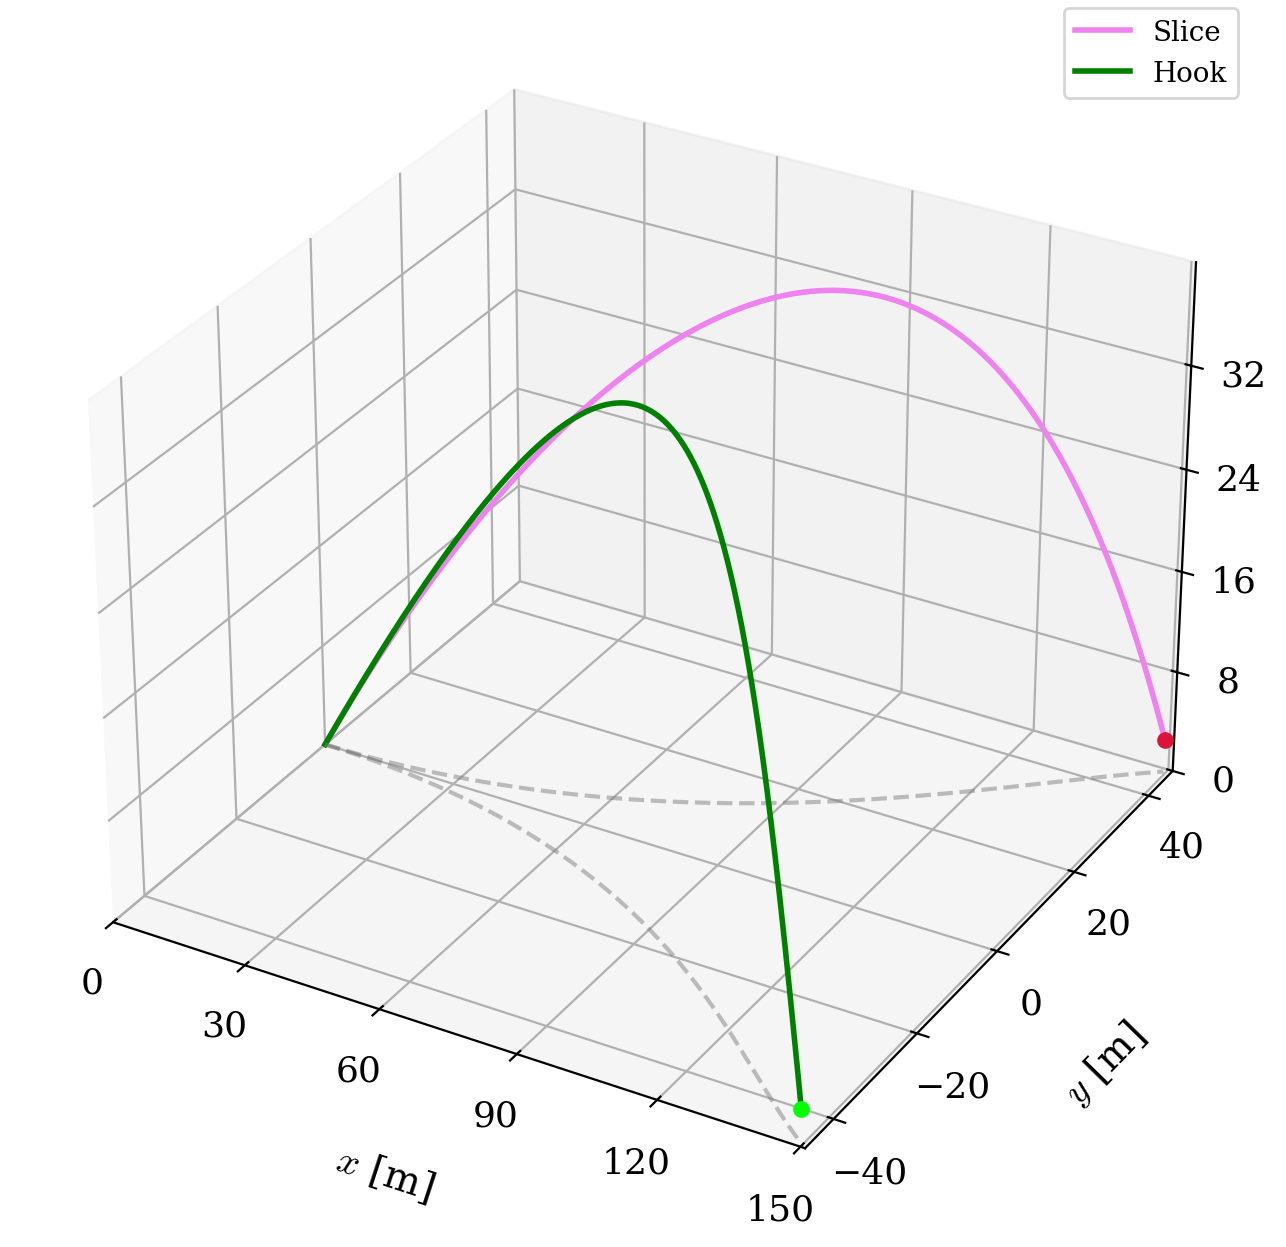
\includegraphics[width=0.55\linewidth]{figures_tex/hook_y_slice.png}}
    
    \caption{Trayectoria de pelota de golf con lanzamiento \textit{slice} y \textit{hook}.}
    \label{fig:hook_slice}
\end{figure}



\subsection{Lanzamiento de Sistema Multicuerpo}
En este apartado se presentan los lanzamientos de dos sistemas multicuerpo unidos por un muelle viscoelástico, formados por 2 y 3 cuerpos respectivamente. Se considera el caso ideal, ya que el objetivo es el comportamiento del sistema al ser lanzado. Sus trayectorias tridimensionales se muestran en las Figuras \ref{fig:2_3d} y \ref{fig:3_3d}, y se encuentran animadas en 
\href{https://www.youtube.com/watch_videos?video_ids=gUw4wHvm8VQ,M7mvM2oSOLI}{YouTube}.




\begin{figure}[h]
    \centering
    \href{https://youtu.be/gUw4wHvm8VQ?list=PLYDzV8MgIoON7YU9Pd_x0HvjzlLKixw87}{
    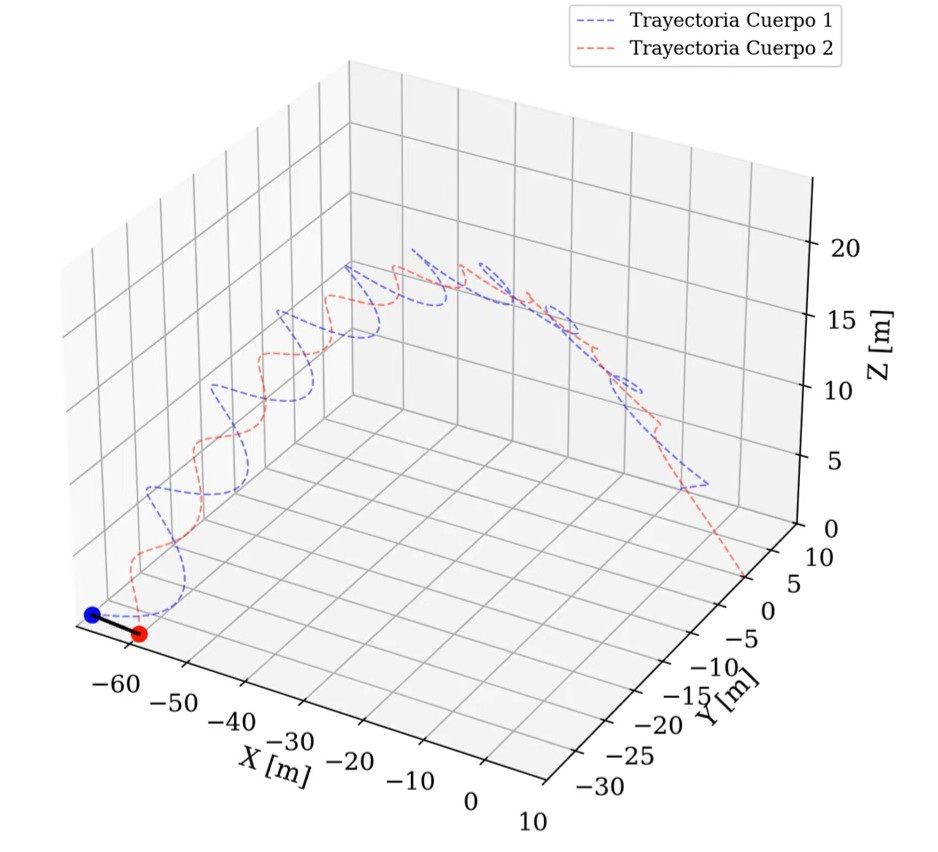
\includegraphics[width=0.55\linewidth]{figures_tex/2_3d.jpeg}}
        \caption{Trayectoria sistema 2 cuerpos unidos por muelle viscoelástico.}
    \label{fig:2_3d}
\end{figure}

Para el caso de dos cuerpos acoplados mediante un muelle viscoelástico, se observa que el centro de masas describe una trayectoria parabólica balística, mientras que las fuerzas internas provocan una oscilación amortiguada y una rotación relativa, resultando en un patrón helicoidal para cada masa individual,

En la configuración de tres cuerpos, se consideró un modelo de ``suelo transparente'' al omitir la detección de colisiones con el plano $z = 0$, permitiendo que el sistema evolucione en caída libre indefinida. El sistema aumenta en complejidad y traza una trayectoria errática al comienzo (solución transitoria) hasta finalmente lograr una trayectoria cuasiperiódica por parte de los tres cuerpos (solución estacionaria).


\begin{figure}[h]
        \centering
        \href{https://www.youtube.com/watch?v=M7mvM2oSOLI&list=PLYDzV8MgIoON7YU9Pd_x0HvjzlLKixw87}{ 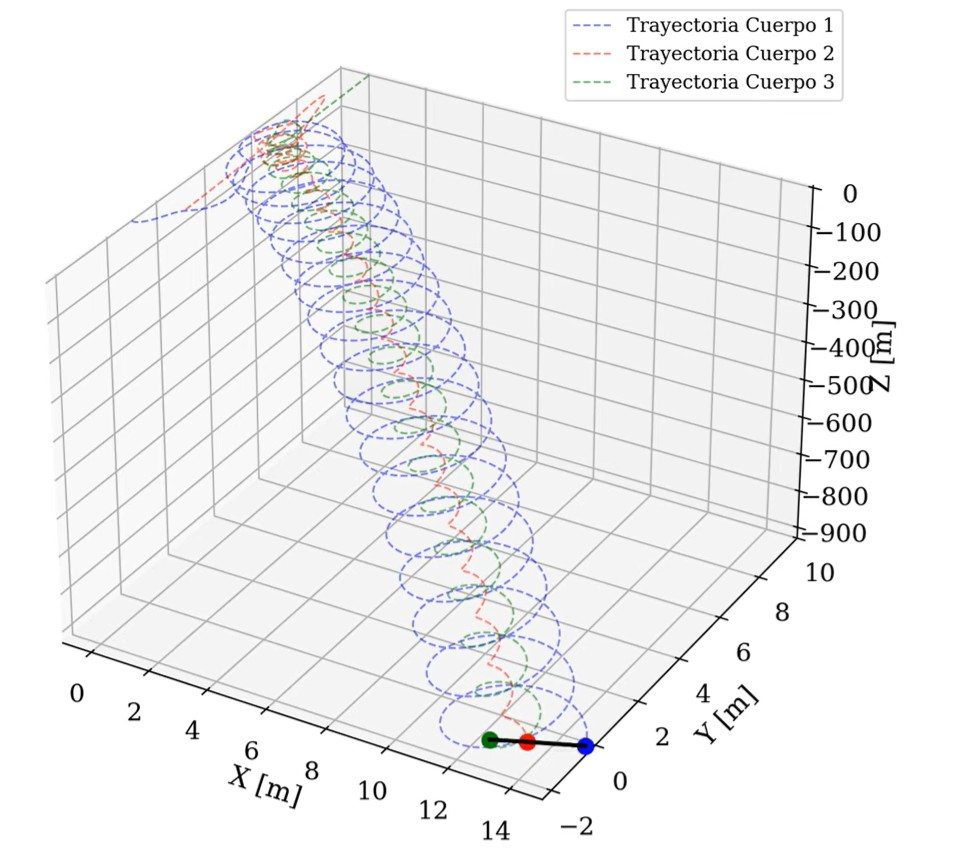
\includegraphics[width=0.55\linewidth]{figures_tex/3_2d.jpeg}}
        \caption{Trayectoria sistema 3 cuerpos unidos por muelles viscoelásticos.}
        \label{fig:3_3d}
    \end{figure}

